\documentclass[11pt]{article}
\usepackage{amsmath,amssymb,booktabs,geometry,graphicx,siunitx}
\usepackage[numbers,sort&compress]{natbib}
\usepackage{placeins}
\usepackage[hidelinks]{hyperref}
\geometry{margin=1in}
\graphicspath{{figures/}}
\title{Verifying FTCS and Crank--Nicolson for a Single Heat-Equation Mode}
\author{Tanner Polley}
\date{}
\begin{document}
\maketitle

\begin{abstract}
This tutorial separates code verification, solution verification, linear
stability, monotonicity, and numerical uncertainty for two finite-difference
schemes applied to a dimensionless one-dimensional heat equation. Compact
claim-bearing tests verify each declared discrete method. Retained refinement
studies recover second-order combined behavior for both methods, first-order
isolated temporal behavior for FTCS, and second-order isolated temporal
behavior for Crank--Nicolson. Case-specific acceptance follows from the
measured refinement regime rather than a generic order band.
\end{abstract}

\section{Question and formulation}

We solve
\begin{equation}
  \frac{\partial\theta}{\partial Fo}
  =\frac{\partial^2\theta}{\partial\xi^2},
  \qquad 0<\xi<1,
\end{equation}
with \(\theta(0,Fo)=\theta(1,Fo)=0\) and
\(\theta(\xi,0)=\sin(\pi\xi)\). All quantities are dimensionless. The
continuous reference is
\begin{equation}
  \theta_{\mathrm{ref}}(\xi,Fo)
  =\exp(-\pi^2Fo)\sin(\pi\xi).
\end{equation}
This case supports code and solution verification. It does not constitute
physical model validation.

\section{Discrete methods and reference oracles}

On a uniform grid, \(r=\Delta Fo/(\Delta\xi)^2\). FTCS updates
\begin{equation}
  \theta_i^{n+1}=\theta_i^n+r
  (\theta_{i-1}^n-2\theta_i^n+\theta_{i+1}^n)
\end{equation}
and requires \(r\leq1/2\). Crank--Nicolson uses
\begin{equation}
\begin{split}
  \theta_i^{n+1}-\theta_i^n=\frac{r}{2}\big[&
  \theta_{i-1}^{n+1}-2\theta_i^{n+1}+\theta_{i+1}^{n+1}\\
  &+\theta_{i-1}^{n}-2\theta_i^n+\theta_{i+1}^n\big].
\end{split}
\end{equation}
Crank and Nicolson present this centered finite-difference form as Method III
in Section 4, equation (16), printed pages 54--55
\citep{crankPracticalMethodNumerical1947}. Their Section 7(b), printed page 59,
discusses damping of Method III error modes and slowly disappearing oscillation
for a large step ratio.

For phase \(\mu\), independent substitution gives
\begin{align}
  G_{\mathrm{FTCS}}&=1-4r\sin^2(\mu/2),\\
  G_{\mathrm{CN}}&=\frac{1-2r\sin^2(\mu/2)}
                         {1+2r\sin^2(\mu/2)}.
\end{align}
These factors verify discrete-mode behavior, while the continuous reference
verifies solution convergence. An exact-in-time centered-space reference
isolates temporal error.

\section{Code verification}

The installable Python package implements FTCS directly and solves the
Crank--Nicolson tridiagonal system with SciPy. Seven compact tests protect the
continuous reference, exact boundaries, independent discrete-mode
amplification for both solvers, FTCS stability rejection, the distinction
between stability and monotonicity, and combined-refinement entry into the
second-order regime. The tests use allowances derived from binary64 scale and
time-step accumulation, not a repository-wide epsilon.

\section{Solution verification}

All studies end at \(Fo=0.1\). Combined refinement uses
\(N=10,20,40,80,160\) and fixes \(r=0.4\). Isolated temporal refinement holds
\(N=20\), uses 80 through 1280 steps, and compares with the semidiscrete
reference.

\begin{figure}[htbp]
  \centering
  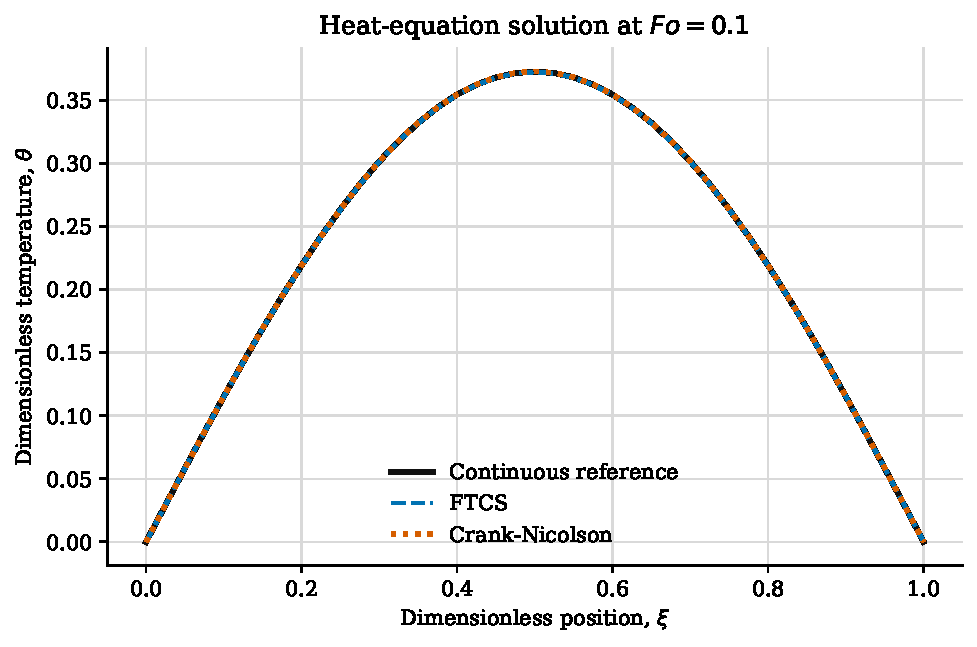
\includegraphics[width=0.78\textwidth]{solution_overlay.pdf}
  \caption{The numerical fields at \(N=40\), \(r=0.4\), and \(Fo=0.1\).
  The close overlay motivates quantitative error metrics rather than visual
  agreement alone.}
  \label{fig:solution}
\end{figure}

\begin{figure}[htbp]
  \centering
  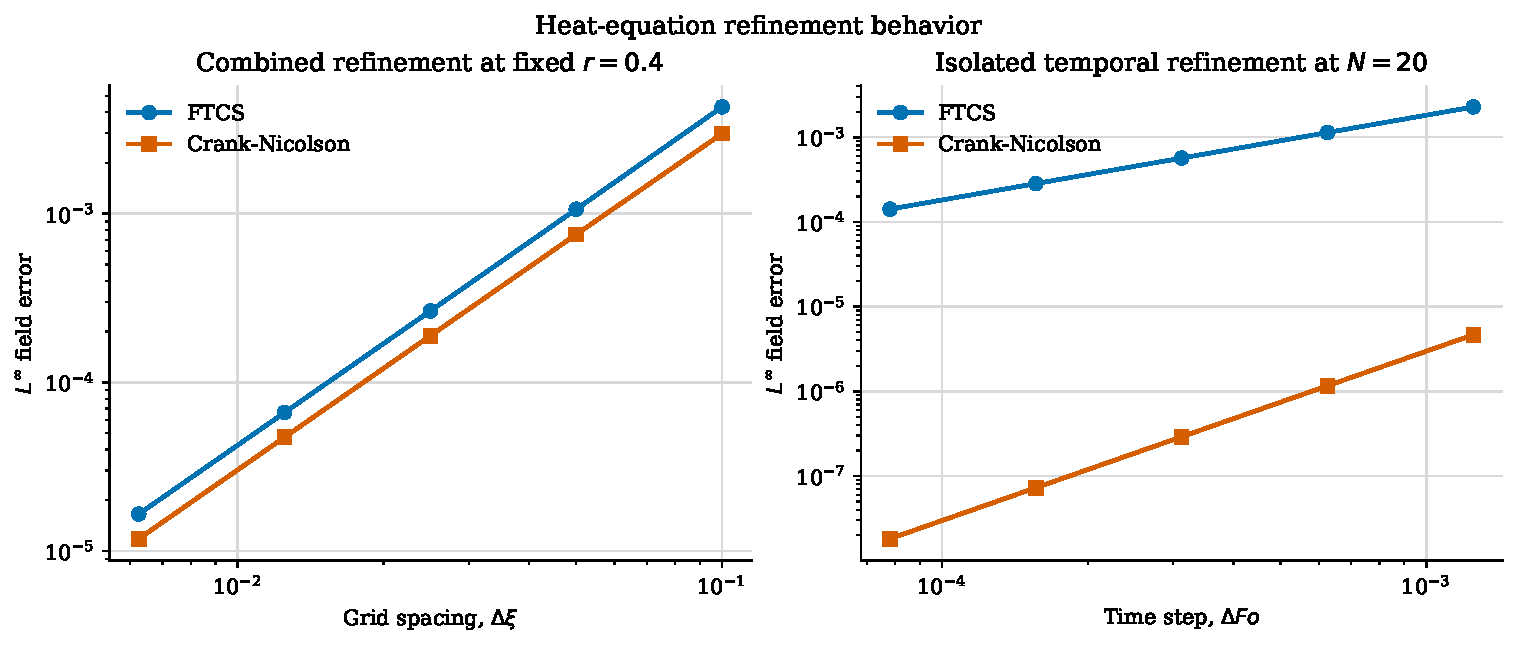
\includegraphics[width=0.82\textwidth]{refinement.pdf}
  \caption{Combined and isolated temporal \(L^\infty\) refinement behavior.
  Every sequence decreases monotonically.}
  \label{fig:refinement}
\end{figure}

\begin{table}[htbp]
\centering
\caption{Finest retained solution-verification results.}
\begin{tabular}{llrrr}
\toprule
Study & Method & \(E_\infty\) & \(p_{\mathrm{obs}}\) & Value bound\\
\midrule
Combined & FTCS & \num{1.654619e-5} & \num{2.000230} & \num{2.068712e-5}\\
Combined & Crank--Nicolson & \num{1.181738e-5} & \num{1.999746} & \num{1.476826e-5}\\
Temporal & FTCS & \num{1.415673e-4} & \num{1.000467} & \num{1.770737e-4}\\
Temporal & Crank--Nicolson & \num{1.814958e-8} & \num{2.000004} & \num{2.268708e-8}\\
\bottomrule
\end{tabular}
\label{tab:results}
\end{table}

The combined path makes the FTCS time error and centered-space error scale as
\((\Delta\xi)^2\). Crank--Nicolson's temporal contribution is higher order on
that path, so its spatial term controls the asymptotic rate. Removing spatial
error with the semidiscrete reference recovers the expected first- and
second-order temporal rates.

\section{Stability and monotonicity}

\begin{figure}[htbp]
  \centering
  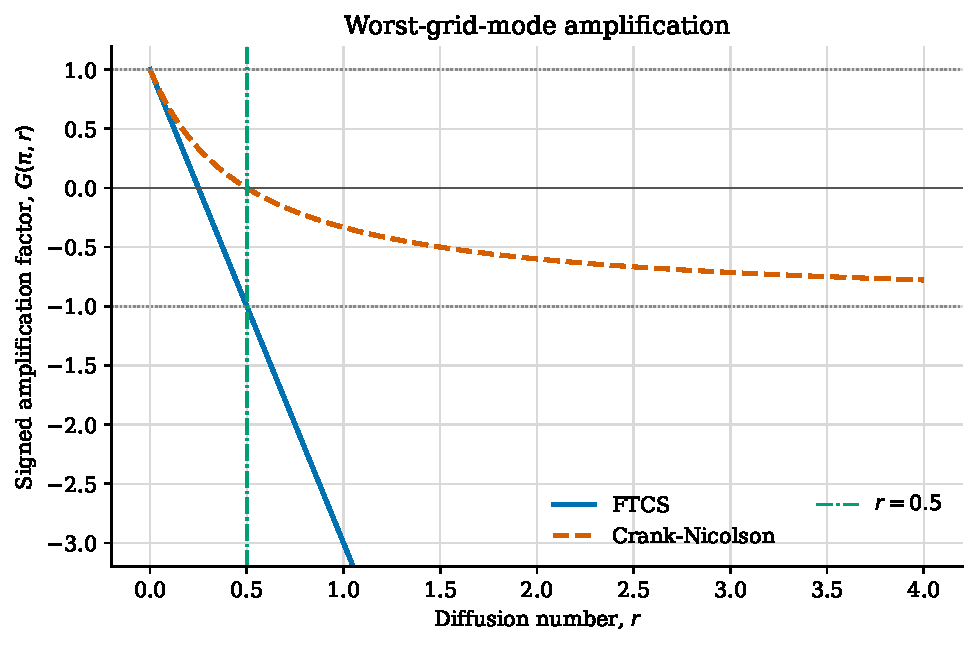
\includegraphics[width=0.68\textwidth]{amplification.pdf}
  \caption{Worst-grid-mode amplification. FTCS crosses \(G=-1\) at
  \(r=0.5\). Crank--Nicolson remains bounded but changes sign, allowing
  decaying alternation.}
  \label{fig:amplification}
\end{figure}

Figure~\ref{fig:amplification} makes two claims visible without merging them.
FTCS is unstable above its stated limit. Crank--Nicolson is linearly stable for
positive \(r\), but it is not unconditionally monotone.
\FloatBarrier

\section{Numerical uncertainty and acceptance}

For target order \(p\), the fine-grid acceptance bound is
\begin{equation}
  U_h=1.25\frac{\|\theta_{h/2}-\theta_h\|_\infty}{2^p-1}
  +64\epsilon_{64}\max(1,\|\theta_{h/2}\|_\infty).
\end{equation}
Every finest error in Table~\ref{tab:results} is below its bound. The order
tolerance is twice the change between the two finest observed orders plus the
propagated floating allowance. The largest retained Crank--Nicolson linear
residual is \(4.44\times10^{-16}\), far below discretization error.

\section{Limitations and reproduction}

The evidence covers one smooth mode, a uniform one-dimensional grid, constant
coefficients, and exact homogeneous boundaries. It does not cover nonsmooth
fields, variable coefficients, nonlinear sources, multidimensional operators,
or physical uncertainty.

From a fresh checkout, run:
\begin{quote}
\small\ttfamily
uv sync\\
uv run python scripts/validate\_project.py full
\end{quote}
The validation ladder regenerates tables and figures, checks the project-only
Zotero bibliography, recomputes acceptance, runs tests, and rebuilds this
manuscript.

\bibliographystyle{plainnat}
\bibliography{references}
\end{document}
